\section{Software architecture views}
\subsection{Subsystem decomposition}

\newpage
\subsection{Hardware/software mapping}
In this section the hardware/software mapping Tygron uses will be explained, as well as the way our agent will be connected to this.

\subsubsection{Tygron}
Tygron has its own server, from which it communicates with all other entities. For each group of users, there is a seperate server which contains their world and on which those users can work. The general Tygron server knows these other servers and will redirect the user to the particular server. So, when a customer wants to connect to Tygron, it will first connect to this general server. Also, this general server has contact with other servers which are not connected to Tygron. For example, when a customer wants to build a part of a city to play on, the general server will connect to some other servers that give information about this place, like where the buildings are and what the use of those buildings is. 

\subsubsection{Our project}
In our project we have our own server with all TU Delft students. But there is another thing that needs to be different: the way we connect to that server. Since we don't use humans, but agents to play the game, those agents need to connect in some way to the server. To do so we have a connector between our instance and the server. This connector will use the goal code we wrote and will translate this into actions in the game. This way our agent can play the game. The next picture illustrates this.

\begin{center}
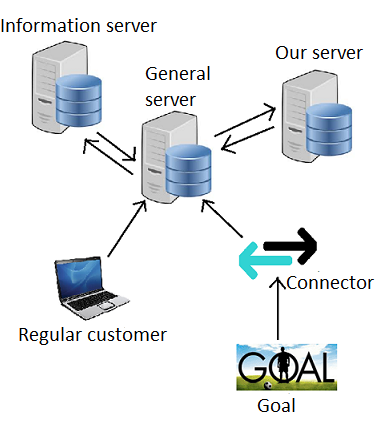
\includegraphics[scale=0.68]{Server_model.png}
\end{center}

\subsection{Persistent data management}
\subsection{Concurrency}





